
\documentclass{article} % For LaTeX2e
\usepackage[preprint]{colm2026_conference}

\usepackage{microtype}
\usepackage{hyperref}
\usepackage{url}
\usepackage{graphicx}
\usepackage{booktabs}
\usepackage[textsize=small]{todonotes}
\usepackage{amsmath}
\usepackage{cleveref}
\usepackage{amsthm}
\usepackage{algorithm}      
\usepackage{algorithmicx}   
\usepackage{algpseudocode}
\usepackage{amssymb}
\usepackage{cleveref}
\usepackage{subcaption}

% NOTE: including geometry package
% The geometery package modifies some page properties when used. This can dramatically change the page margins, leading to severe template violation, and potential desk rejection. If the package is required, it can be used with the "pass" flag to skip the default page modifications, as in the following line:
% \usepackage[pass]{geometry}

\usepackage{lineno}

\definecolor{darkblue}{rgb}{0, 0, 0.5}
\hypersetup{colorlinks=true, citecolor=darkblue, linkcolor=darkblue, urlcolor=darkblue}

% Theorem-like environments
\newtheorem{assumption}{Assumption}[section]
\newtheorem{theorem}{Theorem}[section]
\newtheorem{lemma}[theorem]{Lemma}
\newtheorem{proposition}[theorem]{Proposition}
\newtheorem{corollary}[theorem]{Corollary}
\theoremstyle{definition}
\newtheorem{definition}[theorem]{Definition}
\theoremstyle{remark}
\newtheorem{remark}[theorem]{Remark}

% Define custom todonotes for different purposes:
\newcommand{\fixme}[1]{\todo[inline,color=red!40]{TODO: #1}}
\newcommand{\note}[1]{\todo[inline,color=blue!40]{NOTE: #1}}
\newcommand{\improve}[1]{\todo[inline,color=green!40]{IMPROVE: #1}}
 
\newcommand{\junda}[1]{\textcolor{purple}{~\textbf{Junda}:~#1}}

\newcommand{\tong}[1]{\textcolor{purple}{~\textbf{Tong}: (optional)~#1}}

\title{Skill-R1: Agent Skill Evolution via Reinforcement Learning}

% Authors must not appear in the submitted version. This should be be taken care of automatically as long as you are using the "submission" option for the colm2026_conference package. But it's on the authors to verify. Non-anonymous submissions will be rejected without review.

\author{
Yash Vishe$^{1}$, Rohan Surana$^{1}$, Xunyi Jiang$^{1}$, Zihan Huang$^{1}$, Xintong Li$^{1}$, Nikki Lijing Kuang$^{1}$, \\
\textbf{Tong Yu$^{2}$, Ryan A. Rossi$^{2}$, Jingbo Shang$^{1}$, Julian McAuley$^{1}$, Junda Wu$^{1}$}
\\
$^{1}$UC San Diego \quad
$^{2}$Adobe Research \\
\texttt{\{yvishe,rsurana,xuj003,zih043,xil240,jshang,jmcauley,juw069\}@ucsd.edu} \\
\texttt{\{tyu,ryan.rossi\}@adobe.com} \\
}

% The \author macro works with any number of authors. There are two commands
% used to separate the names and addresses of multiple authors: \And and \AND.
%
% Using \And between authors leaves it to \LaTeX{} to determine where to break
% the lines. Using \AND forces a linebreak at that point. So, if \LaTeX{}
% puts 3 of 4 authors names on the first line, and the last on the second
% line, try using \AND instead of \And before the third author name.

\newcommand{\fix}{\marginpar{FIX}}
\newcommand{\new}{\marginpar{NEW}}

\begin{document}

\ifcolmsubmission
\linenumbers
\fi

\maketitle


% Here is my abstract contents brainstorm draft. The methodology design is illustrated in the figure. Please based on my abstract content and the figure, provide a formal abstract and a contribution list of 4 bullet points to present the story. I want the writing to be major machine learning conference paper styles, like NIPS, ICLR, ICML.

% \begin{abstract}

% 1. Background: Agent skills advanced LLM agents (in introduction, we need to expand on Anthropic use cases and more references)
% 2. Limitation 1: Agent skills are mostly pre-defined and lack an adaptive way to improve through previous trials and errors (we need references in the intro)
% 3. Limitation 2: Agent skills are limited to a set of reusable skills that cannot be tailored to individual tasks' scenarios. (references in intro)
% 4. To bridge the limitations, we propose Skill-R1, which enables agent skill self-evolution through reinforcement learning from verifiable rewards.
% 5. Design 1: We enable a skill generator which summarizes prevously rollouted trajectories with previously generated skills as conditions, learns from the trails and errors (possitive and negative verifiable rewards), and recurrently generate "next generation" of rollouts. (Please read my illustration figure and the response to small-LLLM loop is recurrent and can generate several genrations of rollout groups)
% 6. Design 2: To further enable GRPO for parameter updates, we identify bi-level group advantages which are both the advantages among the group of a certain generation of rollouts, as well as next generation advantages (inter-generation groups.). (Please read my illustration figure. Also please help me better illustrate this in an intuitive evoluationary narrative.)

% Please note to link Designs to limitations.

% \end{abstract}


% \begin{abstract}
% Agentic large language models often rely on skills, reusable natural language procedures that condition how the agent plans, acts, and uses tools.
% In conventional systems, agent skills are either predefined or updated without an explicit trial-and-error loop on the current task instance, 
% which can limit adaptivity and instance-level specialization. 
% We propose \textbf{Skill-R1}, a reinforcement learning framework that enables skills to evolve from verifiable rewards through an iterative generate evaluate update process.
% \textbf{Skill-R1} introduces an evolutionary rollout mechanism that organizes interaction into multiple generations. 
% In each step of skill evolution, a lightweight skill generator conditions on the task context together with previously collected rollouts and their verified outcomes,
% synthesizes updated skills, and injects them as conditioning into a task LLM to produce a new generation of rollouts. 
% Verified rewards act as selection signals over the updated skills, and the resulting successes and failures provide supervision for producing the next generation of skills.
% This recurrent design targets instance-level adaptation by self-evolution of skills to the observed error patterns and progress signals on the current task.
% To optimize the skill generator from these evolutionary rollouts, we develop a bi-level group relative policy optimization objective 
% that combines \textit{intra-generation} and \textit{inter-generation} advantages. 
% The intra-generation advantage compares rollouts within the same generation to capture relative quality under shared conditioning.
% The inter-generation advantage measures improvement across successive generations to encourage progress in the evolving skill conditioned rollout distribution.
% Importantly, the task LLM is treated as a frozen black box and can be either closed or open,
% making \textbf{Skill-R1} model agnostic while still enabling reinforcement learning updates to the skill generator.
% Empirically, we evaluate \textbf{Skill-R1} on agent tasks with programmatically verifiable outcomes and observe consistent gains over fixed skill baselines and single generation self refinement variants, along with analyses that isolate the roles of multi generation evolution and bi-level advantages.
% \end{abstract}


\begin{abstract}
Agentic large language models often rely on skills, reusable natural-language procedures that guide planning, action, and tool use.
In practice, however, skills are typically improved through prompt engineering or by aligning the task LLM itself to revised skills, 
which is costly, model-specific, and often infeasible for closed-source models.
Meanwhile, skill optimization is not a one-step prompt engineering problem, but a recurrent process with two coupled levels of credit assignment.
% \tong{Might it be helpful to clarify in the abstract what makes this recurrent process technically challenging or non-trivial to solve?}
A useful skill must improve rollout quality under the current conditioning, while a useful revision must turn observed successes and failures into a better skill for the next round.
We therefore formulate skill evolution as a bi-level optimization problem over rollout selection within each generation and skill improvement across generations.
We propose \textbf{Skill-R1}, a reinforcement learning framework for instance-level recurrent skill optimization from verifiable rewards.
Rather than updating the task LLM, \textbf{Skill-R1} trains a lightweight skill generator that conditions on the task context, 
prior rollouts, and their verified outcomes to produce skills that steer a frozen task LLM.
This design preserves black-box compatibility with both open- and closed-source models while making adaptation substantially cheaper than model-level updates.
\textbf{Skill-R1} proceeds over multiple generations. At each generation, the current skill induces rollouts from the task LLM, whose verified outcomes are fed back to produce the next revision.
To optimize the skill generator over this recurrent process, we introduce a bi-level group-relative policy optimization objective with \textit{intra-generation} and \textit{inter-generation} advantages.
The intra-generation term compares rollouts under shared skill conditioning, while the inter-generation term rewards revisions that improve the induced behavior over successive generations.
Together, these terms provide a principled objective for directional skill evolution rather than one-shot or heuristic self-refinement.
% \tong{Might it be helpful to clarify in the abstract how the bi-level decomposition specifically addresses the technical challenges of recurrent skill optimization?}
% \fixme{
% Empirically, on agent tasks with programmatically verifiable outcomes, \textbf{Skill-R1} consistently outperforms fixed-skill baselines and single-generation self-refinement variants. Further analysis isolates the benefits of multi-generation evolution and the proposed bi-level advantages.
% }
Empirical evaluations suggest that Skill-R1 achieves consistent improvements over both no-skill baselines and standard GRPO across benchmarks with verifiable rewards. The gains are particularly strong on complex, multi-step tasks, where single-pass refinement methods struggle.
\end{abstract}



% The LONG VERSION
% \begin{abstract}
% Agentic large language models often rely on skills, reusable natural language procedures that shape how the agent plans, acts, and uses tools.
% Yet skill adaptation in current systems remains limited: skills are often fixed in advance, revised through heuristic prompt engineering or LLM-based rewriting, or improved only by adapting the underlying task LLM itself, which is costly, model-dependent, and often infeasible for closed-source models.
% Moreover, effective skill improvement is inherently sequential.
% A useful skill update should not only produce stronger rollouts under the current skill conditioning, but also correct the failure modes of earlier attempts and drive sustained progress on the current task instance.
% Existing skill self-evolution pipelines rarely provide a principled optimization mechanism for this process, leaving both the direction and efficiency of skill improvement weakly controlled.

% We propose \textbf{Skill-R1}, a reinforcement learning framework for instance-level skill evolution from verifiable rewards through an iterative generate-evaluate-update process.
% Rather than adapting the task LLM, \textbf{Skill-R1} learns a lightweight skill generator that conditions on the task context together with previously collected rollouts and their verified outcomes, and synthesizes updated skills to condition a frozen task LLM.
% This design preserves black-box compatibility with both open- and closed-source task LLMs while making skill adaptation substantially cheaper than model-level updates.

% To support sequential skill improvement, \textbf{Skill-R1} introduces an evolutionary rollout mechanism that organizes interaction into multiple generations.
% At each generation, the updated skill induces a new rollout distribution from the task LLM, and the resulting successes and failures are fed back as supervision for the next skill revision.
% This recurrent design enables skills to evolve in response to observed error patterns and progress signals on the current instance, rather than remaining static or relying on one-shot self-refinement.

% To optimize the skill generator from these evolutionary rollouts, we develop a bi-level group-relative policy optimization objective that combines \textit{intra-generation} and \textit{inter-generation} advantages.
% The intra-generation advantage compares rollouts within the same generation to capture relative quality under shared skill conditioning.
% The inter-generation advantage measures improvement across successive generations, explicitly encouraging updated skills to move the induced rollout distribution toward higher-reward behaviors over time.
% Together, these two levels of advantage provide a principled optimization strategy for skill evolution that rewards both local relative quality and global progress across revisions.

% Empirically, we evaluate \textbf{Skill-R1} on agent tasks with programmatically verifiable outcomes and observe consistent gains over fixed-skill baselines and single-generation self-refinement variants, together with analyses that isolate the contributions of multi-generation evolution and bi-level advantages.
% \end{abstract}
\section{Introduction}

% \paragraph{Skills as a practical interface for agent behavior.}
Agentic large language models increasingly rely on external skills~\citep{xu2026agent,jiang2026sok,chen2026cua,nguyen2025guisurvey,huang2025towardsagentic}, 
which are reusable natural-language procedures that specify how an agent should decompose a task, invoke tools, and verify intermediate results. 
Since skills are designed as complementary modules of the task language model, 
they provide a practical interface for shaping LLM behavior without updating the task language model. 
This separation is practical in realistic deployments, where the task model may be proprietary~\citep{gao2025survey,huang2025surveyfoundation}, 
expensive to adapt~\citep{zhou2025memento,wu2024personalizedmllm,wu2025mitigatingforget,wang2025selfupdatable,zhang2024personalizationsurvey}, or shared across many downstream tasks~\citep{li2026organizing,chen2026skillcraft,jiang2026xskill}.

% \paragraph{The challenge of recurrent instance-level skill improvement.}
However, many skill-based systems rely on well-engineered skills as predefined and fixed artifacts, 
or revise them only through prompting and single-round self-refinement~\citep{jiang2026sok,xu2026agent,chen2026cua,jiang2026xskill,chen2026skillcraft,xia2026skillrl,zhang2026memskill}. 
These strategies can be misaligned and inefficient, since they rely on repeated prompt edits and are not directly aligned with downstream rewards~\citep{wu2025incontext,kveton2025activedpo,xia2025surveyactive}.
On the other hand, some recent works adapt the task language model to the skill by fine-tuning the task language model on the skill~\citep{wang2025reinforcement,li2025commit,wang2024instructgraph},
but this approach can be computationally costly and limited in adaptivity to many downstream tasks~\citep{zhou2025memento,xia2026skillrl,jiang2026adaptationagenticaisurvey,wu2025mitigatingforget,yao2024federatedllm}.
Moreover, skill optimization should not be a single prompt-editing step, but a recurrent decision problem: 
a useful skill should improve rollout quality under the current context, 
and a useful revision should transform observed successes and failures into a better skill for the next round. 
This naturally leads to a bi-level optimization objective that couples execution quality within each generation with skill improvement across generations.
% \tong{Might it be helpful to explain in the introduction why existing single-level optimization approaches (e.g., standard RL or GRPO) are insufficient for this recurrent skill optimization problem?}

% \paragraph{Overview of Skill-R1.}
To address this problem, we propose \textbf{Skill-R1}, a reinforcement learning framework for recurrent agent skill evolution from verifiable rewards. 
\textbf{Skill-R1} separates \emph{task execution} from \emph{skill improvement}. 
A frozen task LLM produces rollouts conditioned on the current skill, 
while a lightweight skill generator is trained to revise that skill based on the task context, prior rollouts, and their verified outcomes~\citep{xia2025knowledgequery,wang2025dice,vannguyen2025smallsurvey}. 
By updating only the skill generator, the framework remains compatible with both open- and closed-source task models and can be more efficient than updating the task model itself~\citep{vannguyen2025smallsurvey,xia2025surveyactive}.

% \paragraph{Evolutionary rollouts across generations.}
The core interaction loop of \textbf{Skill-R1} is multi-generation. 
For a given instance, the current skill induces a group of rollouts from the frozen task model, a verifier scores these rollouts, and the resulting trials and errors~\citep{wu2025ocean, wu2024decot},
and reward signals are appended to an instance-specific history that conditions the next skill revision. 
Recurring execution of this process yields an evolutionary view of skill improvement, in which each generation proposes a new skill, 
tests it through a rollout population, and passes forward evidence for subsequent refinement.
This recurrent structure makes it possible to optimize directional improvement~\citep{xia2026skillrl,sun2025seagent,zhou2025memento} on the same instance rather than selecting among isolated one-shot attempts.

% \paragraph{Bi-level credit assignment for skill evolution.}
The policy optimization of the skill generator requires both intra-generation and inter-generation credit assignment to optimize the skill generator.
To enable optimization of the recurrent skill generator, we introduce a bi-level group-relative policy optimization~\citep{zhong2026rc,shao2024deepseekmath,mundada2026wsgrpo} objective that mirrors the recurrent structure above. 
The \emph{intra-generation} term compares rollouts sampled under the same skill and captures relative execution quality within a generation. 
The \emph{inter-generation} term measures whether a revised skill improves the average verified performance relative to the previous generation.
Together, these signals provide a principled objective for rewarding both strong rollouts and beneficial skill revisions~\citep{wu2025incontext, surana2026massdpo, li2025impsamplingdpo, huang2025pluralistic}.
% \fixme{Empirical findings}
Our experiments demonstrate that Skill-R1 consistently improves agent performance across diverse reasoning and tool-use benchmarks, outperforming both no-skill baselines and standard GRPO. 
We also show a clear performance gap between skill generations, which demonstrates the effectiveness of the recurrent skill evolution.
% Instead of relying on one-shot edits, Skill-R1 adopts an iterative evolution process guided by execution feedback, enabling more reliable and targeted improvements. The multi-generation framework supports progressive capability building, while the bi-level objective ensures that updates are both locally effective and aligned with longer-term optimization. 
% Furthermore, learning the skill editor plays a critical role by allowing the system to distinguish persistent failure modes from incidental noise, resulting in more stable and transferable skill adaptations.
We summarize the contributions of this work as follows:
\begin{itemize}
    \item We formulate recurrent instance-level skill evolution as a bi-level group-relative policy optimization problem.
    \item We propose \textbf{Skill-R1}, a model-agnostic framework that trains a lightweight skill generator while keeping the task LLM frozen.
    \item We introduce a recurrent multi-generation rollout process together with a bi-level GRPO objective that combines \emph{intra-} and \emph{inter-generation} advantages. 
    % \tong{Might it be helpful to verify that the benefit of combining intra- and inter-generation advantages is demonstrated through ablation studies in the experimental section?}
    \item We evaluate \textbf{Skill-R1} on agent tasks with verifiable rewards, comparing with agent skill and GRPO baselines and achieving superior performance.
    % comparing against fixed-skill and single-generation baselines and isolating the effects of multi-generation evolution and bi-level advantages through ablations.} \tong{It seems that the keyword 'ablation' is only mentioned here in this paper.}
\end{itemize}
\section{Preliminaries}\label{sec:preliminaries}

\subsection{Agent Skills} \label{sec:prelim-skills}
Recent LLM-agent systems commonly treat skills as reusable units of external procedural knowledge that can be retrieved, executed, and updated without modifying the underlying task model. 
Following this practice, let $\pi_{\mathrm{task}}$ denote a frozen task LLM, and let $\mathcal{S}$ be a space of explicit skill artifacts.

\begin{definition}[Agent Skill]
An agent skill is a reusable procedural artifact $s \in \mathcal{S}$ that conditions the execution of the task model on an input instance. 
A skill may encode natural-language instructions, structured workflows, tool-use guidance, or other procedural constraints, while remaining external to the parameters of $\pi_{\mathrm{task}}$.
\end{definition}

Given an instance $x$ and a skill $s$, the frozen task model induces a rollout distribution
\begin{equation} \label{eq:rollout_dist}
\pi_{\mathrm{task}}(\tau \mid x, s),
\end{equation}
where $\tau$ denotes the resulting trajectory. 
In our setting, skills evolve recurrently on the same instance. 
We write $s_g \in \mathcal{S}$ for the skill used at generation $g$, and $\mathcal{H}_g$ for the instance-specific history available up to generation $g$, such as prior rollouts and their verified outcomes. 
These variables will be used to formalize skill evolution in later sections.


\subsection{Group-Relative Policy Optimization} \label{sec:prelim-grpo}
We briefly review Group-Relative Policy Optimization (GRPO) in the language-generation setting, where a policy $\pi_\theta(\cdot \mid x)$ defines a distribution over response rollouts $y$ conditioned on a prompt or context $x \sim \mathcal{D}$. 
GRPO samples a group
\begin{equation} \label{eq:group_sampling}
\mathcal{G}(x)=\{y^{(i)}\}_{i=1}^K,
\qquad
y^{(i)} \stackrel{\mathrm{i.i.d.}}{\sim} \pi_\theta(\cdot \mid x),
\end{equation}
assigns each rollout a verifier score $r(y^{(i)})$, and defines the group-relative advantage
\begin{equation} \label{eq:grpo_adv}
A\!\left(y^{(i)};\mathcal{G}(x)\right)
=
r\!\left(y^{(i)}\right)
-
\frac{1}{K}\sum_{j=1}^K r\!\left(y^{(j)}\right).
\end{equation}
The GRPO objective is
\begin{equation} \label{eq:grpo_obj}
\mathcal{L}_{\mathrm{GRPO}}(\theta)
=
\mathbb{E}_{x \sim \mathcal{D},\, \mathcal{G}(x)}
\left[
\sum_{i=1}^K
A\!\left(y^{(i)};\mathcal{G}(x)\right)
\log \pi_\theta\!\left(y^{(i)} \mid x\right)
\right].
\end{equation}
This group-centered objective promotes rollouts that outperform their peers under the same input context.

\section{Skill-R1: Agent Skill Evolution via Reinforcement Learning}
\label{sec:methodology}

We propose \textbf{Skill-R1} (illustrated in~\Cref{fig:flow}), a reinforcement learning framework that improves a frozen task model by recurrently refining external skills without updating the task model itself.
\textbf{Skill-R1} decouples \emph{task execution} from \emph{skill improvement}: a frozen task LLM generates rollout trajectories conditioned on a selected skill,
while a separate editor policy updates skills based on verified execution outcomes.


% \begin{figure}[H]
%     \centering
%     \includegraphics[width=\linewidth, height=4cm]{figures/phase1.pdf}
    
%     \includegraphics[width=\linewidth, height=4cm]{figures/phase2.pdf}
%     \caption{Overview of Skill-R1. \textbf{Phase 1} iteratively generates skills, rolls out a frozen task LLM, and stores verifier-scored outcomes in an evolutionary history. \textbf{Phase 2} computes a bi-level GRPO advantage from both intra-generation relative performance and inter-generation progress, and uses it to update the skill generator while keeping the task LLM frozen.}
%     \label{fig:flow}
% \end{figure}
\begin{figure}[ht]
\centering 
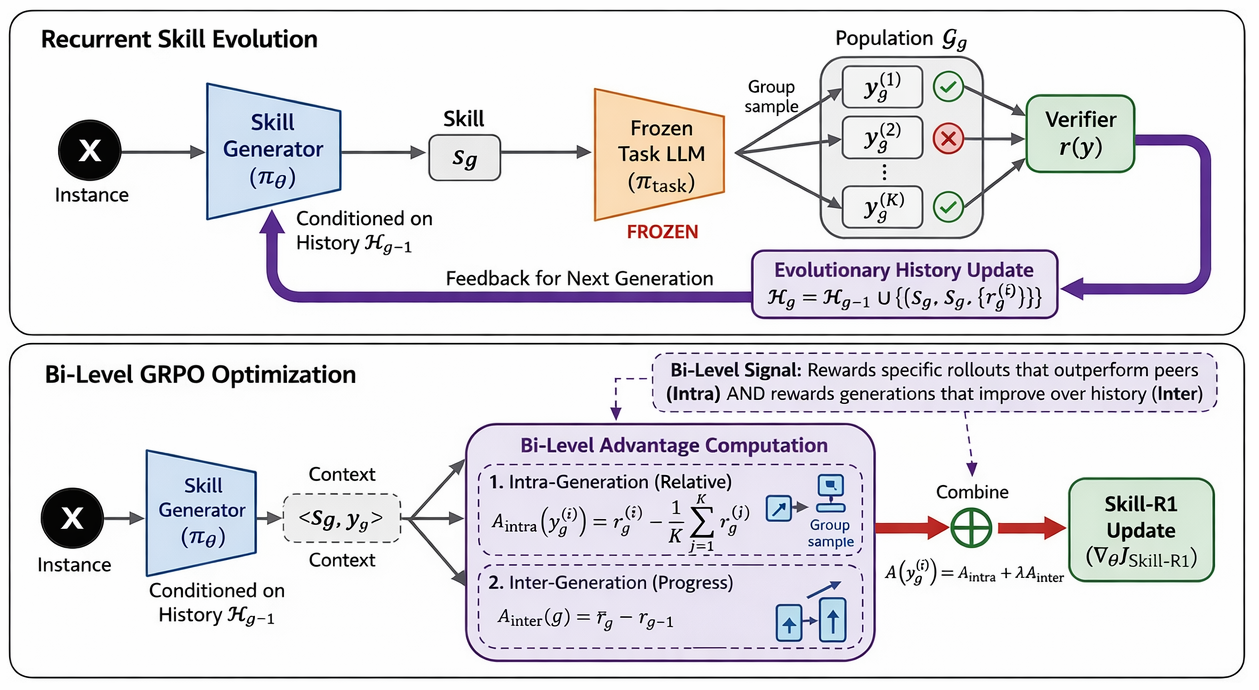
\includegraphics[width=1\linewidth]{figures/fig2-updated.png} 
\caption{Overview of Skill-R1. \textbf{Recurrent Skill Evolution} iteratively generates skills, rolls out a frozen task LLM, and stores verifier-scored outcomes in an evolutionary history. \textbf{Bi-level GRPO Optimization} computes GRPO advantages from both intra-generation relative performance and inter-generation progress, and uses it to update the skill generator while keeping the task LLM frozen.}
\label{fig:flow} 
\end{figure}

\subsection{Problem Setup} \label{sec:method-setup}

Let $x \in \mathcal{X}$ denote a task instance, and let $\mathcal{B}_x \subseteq \mathcal{S}$ denote the skill bank for instance $x$. 
Following \Cref{sec:prelim-skills}, for a selected skill $s_0 \in \mathcal{B}_{x}$, 
the frozen task model $\pi_{\mathrm{task}}$ induces a rollout distribution \Cref{eq:rollout_dist} over trajectories $y^{(i)} \in \mathcal{G}(x,s_0)$ group sampled (in \Cref{eq:group_sampling}) under skill conditioning, 
while a verifier $f_X:\mathcal{G}(x,s_0)\to\mathbb{R}$ assigns each rollout a scalar reward $r^{(i)}$. 
We also maintain the generation-wise history
\begin{equation} \label{eq:history_init}
\mathcal{H}_0 = \{(x, s_0,y^{(i)},r^{(i)})\}_{i=1}^{K},
\qquad 
y^{(i)} \sim \pi_{\mathrm{task}}(\cdot \mid x, s_0), 
\qquad
i=1,\dots,K.
\end{equation}
Thus, the instance-level performance induced by $s_0$ is determined by the rollout policy and verifier jointly,
and our goal is to improve performance on the given instance by revising skills so that later rollout populations achieve higher verifier reward.

For each generation $g \ge 1$, a learnable skill generator $\pi_\theta$ produces the next skill conditioned on the current instance and the accumulated history:
\begin{equation} \label{eq:skill_gen}
\tau = \{(s_g,\mathcal{G}_g(x,s_g),\{r_g^{(i)}\}_{i=1}^{K})\}_{g=1}^{G},
\qquad
s_g \sim \pi_\theta(\cdot \mid x, \mathcal{H}_{g-1}),
\qquad g=1,\dots,G.
\end{equation}
This defines a recurrent skill-evolution process in which each generated skill is evaluated through the rollout population it induces under the frozen task model \Cref{eq:rollout_dist}, 
and the resulting verifier outcomes are appended to the history to guide subsequent revisions. 
Then the recurrent skill evolution problem can be defined as optimizing $\pi_\theta$ to maximize verifier reward across the entire recurrent process:
\begin{equation} \label{eq:rl_objective}
J(\theta)
=
\mathbb{E}_{x \sim p(x)}
\mathbb{E}_{\substack{
s_g \sim \pi_\theta(\cdot \mid x, \mathcal{H}_{g-1}),\:
y_g^{(i)} \sim \pi_{\mathrm{task}}(\cdot \mid x, s_g)
}}
\left[
\sum_{g=1}^{G}
\gamma^{g-1}
\frac{1}{K}
\sum_{i=1}^{K} r_g^{(i)}
\right].
\end{equation}
Directly optimizing the objective in \eqref{eq:rl_objective} is challenging because the reward signal is evaluated on the task model's rollouts rather than directly on the generated skill. 
To address this structural decoupling between skill generation and task execution, we extend the standard GRPO framework to a bi-level setting. 
In the following section, we formulate a bi-level GRPO objective and derive \emph{bi-level advantages}. 
This formulation allows us to properly assign credit to the skill generator $\pi_\theta$ based on the relative, aggregate performance of the rollout populations that each skill induces.

% \todo[inline]{
% write about how we initialize the skill bank:
% In practice, the skill bank is initialized from a small seed set and then refined online. The episodic memory stores compact summaries of selected skills, rollout outcomes, mean rewards, and extracted success/failure patterns, and is shared by both the selector and the editor. The editor itself can operate in two modes: in \emph{inference mode}, the frozen task model proposes skill revisions from rollout evidence; in \emph{training mode}, a smaller trainable language model serves as the editor and provides token-level log-probabilities for policy optimization.
% }

% \todo[inline]{
% \textbf{MCMC interpretation of self-sampling.}
% A useful theoretical lens for the recurrent self-sampling process is Markov Chain Monte Carlo.
% For a fixed instance $x$, define the skill value
% \begin{equation}
% J(s;x) := \mathbb{E}_{y \sim \pi_{\mathrm{task}}(\cdot \mid x,s)}[\,r(y)\,],
% \label{eq:skill-value-main}
% \end{equation}
% and consider the associated energy-based target distribution over skills
% \begin{equation}
% p^\star_\beta(s \mid x) \propto \exp\!\big(\beta J(s;x)\big), \qquad \beta>0.
% \label{eq:skill-target-main}
% \end{equation}
% When $\beta$ is large, $p^\star_\beta(\cdot\mid x)$ concentrates on skills that maximize $J(s;x)$, which formalizes the notion of a ``best'' skill for the frozen task model on the current instance.
% In classical MCMC, one constructs a Markov chain whose stationary distribution equals $p^\star_\beta$ by using a proposal kernel and an acceptance rule that enforces detailed balance.
% While Skill-R1 does not explicitly implement an accept--reject mechanism, the target in
% \Cref{eq:skill-target-main} clarifies what it means for iterative self-sampling to concentrate on high-value skills.
% }

% \todo[inline]{
% \textbf{Stationary-limit and tracking bound.}
% Skill-R1 uses population rollouts to obtain Monte Carlo evidence about $J(s;x)$ and updates the skill proposal distribution
% $\pi_\phi$. Concretely, in generation $g$ the population mean reward
% \begin{equation}
% \widehat{J}_g := \frac{1}{K}\sum_{i=1}^K r\!\left(y^{(g,i)}\right)
% \label{eq:mc-estimator-main}
% \end{equation}
% estimates $J(s_g;x)$ for the sampled skill $s_g$, and the GRPO update increases the probability of proposing skills that
% yield larger $\widehat{J}_g$. Although $\phi$ changes across generations and the overall process is not a fixed-kernel MCMC,
% we can still make two precise statements.
% First, if the skill generator parameters converge, $\phi_g \to \phi^\star$, then the induced sampling distribution over
% skills becomes stationary at the limit, yielding a well-defined asymptotic proposal distribution for the instance.
% Second, when the parameter drift per generation is small, the induced sampling dynamics can be controlled by a tracking
% bound that quantifies how close the skill sampling distribution is to the stationary distribution of the corresponding
% frozen kernel. We formalize these statements and provide proof sketches in Appendix~\ref{app:mcmc_view}.
% }



\begin{algorithm}[ht]
\caption{Skill-R1: Agent Skill Evolution via Reinforcement Learning}
\label{alg:skillr1}
\begin{algorithmic}[1]
\Require Task distribution $p(x)$, frozen task LLM $\pi_{\mathrm{task}}$, skill generator $\pi_\theta$, initial skill bank $\mathcal{B}$, verifier $f$, generations $G$, group size $K$, mixing coefficient $\lambda$
\For{each task instance $x \sim p(x)$ and its skill bank $\mathcal{B}_x$}
    \State Select initial skill $s_0 \in \mathcal{B}_x$
    \State Sample rollouts $\mathcal{G}_0(x, s_0) = \{y_0^{(i)}\}_{i=1}^K$ from $\pi_{\mathrm{task}}(\cdot \mid x, s_0)$
    \State Score $r_0^{(i)} = f(y_0^{(i)})$ for each $i$; initialize $\mathcal{H}_0 = \{(x, s_0, y_0^{(i)}, r_0^{(i)})\}_{i=1}^K$
    \For{$g = 1, \dots, G$}
        \State Generate skill $s_g \sim \pi_\theta(\cdot \mid x, \mathcal{H}_{g-1})$ \Comment{\Cref{eq:skill_gen}}
        \State Sample rollouts $\mathcal{G}_g(x, s_g) = \{y_g^{(i)}\}_{i=1}^K$ from $\pi_{\mathrm{task}}(\cdot \mid x, s_g)$
        \State Verify $r_g^{(i)} = f(y_g^{(i)})$ for each $i$
        \State Compute $A_{\mathrm{intra}}(y_g^{(i)})$, $A_{\mathrm{inter}}(g)$, and $A(y_g^{(i)})$ \Comment{\Cref{eq:intra_adv,eq:inter_adv,eq:bilevel_adv}}
        \State Update $\mathcal{H}_g = \mathcal{H}_{g-1} \cup \{(s_g, \mathcal{G}_g, \{r_g^{(i)}\}_{i=1}^K)\}$
    \EndFor
\EndFor
\State Update $\theta$ by maximizing $\mathcal{L}_{\mathrm{Skill\text{-}R1}}(\theta)$ over accumulated rollouts \Comment{\Cref{eq:skillr1_obj}}
\end{algorithmic}
\end{algorithm}



\subsection{Bi-Level Group-relative Advantages }
\label{sec:method-advantage}

The reward signal in \Cref{eq:rl_objective} is evaluated on rollouts from the frozen task model, yet the trainable parameters reside in the skill generator $\pi_\theta$.
To route rollout-level feedback to the skill that induced it, we decompose credit assignment into two complementary advantage signals.
Within generation $g$, all $K$ rollouts share the same skill $s_g$, so we apply the group-relative comparison from \Cref{eq:grpo_adv} directly:
\begin{equation} \label{eq:intra_adv}
A_{\mathrm{intra}}(y_g^{(i)})
=
r_g^{(i)} - \frac{1}{K}\sum_{j=1}^K r_g^{(j)}.
\end{equation}
Centering by the group mean makes this signal invariant to absolute reward scale and isolates rollout quality from skill quality.
However, $A_{\mathrm{intra}}$ is blind to whether a skill revision improved on its predecessor.
To capture cross-generation progress, we define the population mean reward and the inter-generation advantage
\begin{equation} \label{eq:inter_adv}
A_{\mathrm{inter}}(g) = \bar{r}_g - \bar{r}_{g-1}, \qquad \bar{r}_g = \frac{1}{K}\sum_{i=1}^K r_g^{(i)}
\end{equation}
with $A_{\mathrm{inter}}(1)=0$.
A positive value indicates that the revised skill shifted the rollout distribution toward higher reward; a negative value penalizes regressions.
We combine the two signals into a single bi-level advantage:
\begin{equation}
A(y_g^{(i)}) = A_{\mathrm{intra}}(y_g^{(i)}) + \lambda\, A_{\mathrm{inter}}(g),
\label{eq:bilevel_adv}
\end{equation}
where $\lambda \ge 0$ interpolates between pure within-generation GRPO ($\lambda{=}0$) and a regime that additionally rewards cross-generation improvement.

\subsection{GRPO Objective for Skill Evolution}
\label{sec:method-objective}

We optimize $\pi_\theta$ with a clipped GRPO surrogate that aggregates the bi-level advantage across all generations.
Let $\rho_g = \pi_\theta(s_g \mid x, \mathcal{H}_{g-1}) / \pi_{\theta_{\mathrm{old}}}(s_g \mid x, \mathcal{H}_{g-1})$ be the importance ratio between the current and data-collection policies. The \textbf{Skill-R1} objective is
\begin{equation}
\begin{aligned}
\mathcal{L}_{\mathrm{Skill\text{-}R1}}(\theta)
&=
\mathbb{E}_{x \sim p(x)}
\Bigg[
\sum_{g=1}^{G}
\sum_{i=1}^{K}
\min\!\left(
  \rho_g\, A(y_g^{(i)}),\;
  \mathrm{clip}(\rho_g,\,1{-}\epsilon,\,1{+}\epsilon)\, A(y_g^{(i)})
\right)
\\
&\quad
-
\beta\,\mathrm{KL}\!\left(\pi_\theta(\cdot \mid x, \mathcal{H}_{g-1}) \,\|\, \pi_{\mathrm{ref}}(\cdot \mid x, \mathcal{H}_{g-1})\right)
\Bigg],
\end{aligned}
\label{eq:skillr1_obj}
\end{equation}
where $A(y_g^{(i)})$ is the bi-level advantage from \Cref{eq:bilevel_adv}, $\epsilon > 0$ is the clipping radius, and $\beta \ge 0$ weights a KL penalty anchoring the policy near a reference $\pi_{\mathrm{ref}}$.
% The clipped minimum stabilizes updates, while the KL term prevents degenerate collapse.
Summing over $g$ generations couples the objective across the entire recurrent process in \Cref{eq:skill_gen},
and thus $\pi_\theta$ is trained to produce improving skill trajectories rather than isolated single-step revisions.
Because only $\pi_\theta$ is updated, the task LLM $\pi_{\mathrm{task}}$ remains frozen and can be open- or closed-source and no gradients through $\pi_{\mathrm{task}}$ are required.
The full procedure is summarized in \Cref{alg:skillr1}.

\section{Experiments}
\label{sec:experiments}

Our experiments are designed to address three key questions: (1) whether conditioning a frozen task language model on progressively evolving skills yields measurable gains over a no-skill baseline, (2) whether a multi-generation rollout framework provides benefits beyond standard GRPO training~\citep{shao2024deepseekmath}, and (3) whether a trained skill editor outperforms an inference-only editor without gradient-based optimization. 
% \tong{Might it be helpful to include in the experimental section a fourth research question about whether the bi-level advantage decomposition (intra vs. inter) contributes to performance, since this is a core technical contribution claimed in the paper?}
% \subsection{Benchmarks}
% \paragraph{GAIA.} The GAIA benchmark~\citep{mialon2023gaia} consists of 165 real-world question-answering tasks requiring multi-step reasoning over heterogeneous data sources, including PDFs, spreadsheets, images, and web pages. Tasks are organized into three difficulty levels---Level~1 ($n = 53$), Level~2 ($n = 86$), and Level~3 ($n = 26$)---reflecting increasing compositional complexity and the number of reasoning steps involved. Each task admits a single ground-truth answer that is verified programmatically through the GAIA evaluation suite, which supports numeric normalization, list-element matching, and case-insensitive string comparison.

% \paragraph{WebWalker.} The WebWalker benchmark~\citep{wu2025webwalker} evaluates an agent's capacity to navigate and extract information from web pages via multi-hop traversal. Tasks require the agent to follow hyperlinks, parse heterogeneous web content, and synthesize answers across multiple pages. We include this benchmark to assess whether skill evolution transfers beyond file-centric question answering to interactive web navigation settings, thereby testing the generality of the Skill-R1 framework.

% \subsection{Experimental Setup}

% \paragraph{Skill initialization.} The base skills were constructed through a two-stage distillation procedure applied independently to each benchmark. In the first stage, we ran GPT-4o-mini on a seed set of ten tasks drawn from each benchmark and stored the resulting reasoning traces, capturing the model's step-by-step problem-solving process, tool invocations, and intermediate conclusions. Both successful and unsuccessful trajectories were retained to expose a broad range of solution strategies and failure modes. In the second stage, these traces were presented to a powerful LLM (Claude Opus 4.6) with an instruction to identify recurring patterns across the trajectories and abstract them into concise, reusable skill guides suited to each benchmark's task distribution. This procedure yielded nine base skills per benchmark (Tables~\ref{tab:main_results}, ~\ref{tab:webwalker_results} and ~\ref{tab:webwalker_source}). For reproducibility, each Skill-R1 run deep-copies the skill directory into an isolated per-run folder, whereas baseline runs share a read-only copy of the same skill bank.


% \paragraph{Methods.} All our experiments use GPT-4o-mini as task LLM. We evaluate the following configurations, each ablating a different component of the Skill-R1 pipeline:

% \begin{itemize}
%     \item \textbf{No Skills (Baseline).} The task LLM (GPT-4o-mini) solves each task directly without any skill conditioning, isolating the base model's standalone capability on the benchmark.
%     \item \textbf{Vanilla GRPO.} Standard Group Relative Policy Optimization is applied to train the editor without the bi-level advantage decomposition or multi-generation rollout structure. This ablation tests whether conventional RL training alone suffices to improve skill quality.
%     \item \textbf{Memento.} An experience-accumulation baseline that augments the task LLM (GPT-4o-mini) with a persistent memory of prior task-solving trajectories, facilitating the retrieval and reuse of accumulated experience.
%     \item \textbf{Skill-R1 (Inference Editor).} The full multi-generation rollout pipeline including skill selection, episodic memory, and skill editing, but with the editor operating in inference mode using a frozen Qwen model. Skill edits are proposed on the basis of rollout evidence without any gradient-based training, thereby isolating the contribution of the evolutionary rollout structure from learned editing.
%     \item \textbf{Skill-R1 (GRPO Editor).} The complete Skill-R1 framework with a GRPO-trained Qwen editor optimized using bi-level advantages (\Cref{eq:bilevel_adv}). The editor is trained online as skills evolve across generations and tasks, representing the full system.
% \end{itemize}
\subsection{Experimental Setup}
\paragraph{Tasks.}We evaluate Skill-R1 on two benchmarks requiring multi-step reasoning, tool use, and verifiable answers: GAIA~\citep{mialon2024gaia}, which consists of 165 real-world tasks over heterogeneous sources (e.g., PDFs, spreadsheets, and web pages), and WebWalker~\citep{wu2025webwalker}, which focuses on multi-hop web navigation and cross-page reasoning. Together, they capture both structured reasoning and interactive decision-making.

\paragraph{Baselines.} Our baselines are designed to isolate key components of the pipeline. No Skills measures the base model’s standalone capability without skill conditioning. Vanilla GRPO applies standard Group Relative Policy Optimization to train the editor without bi-level advantage decomposition or multi-generation rollouts, evaluating whether conventional RL alone suffices to improve skill quality.

\paragraph{Skill initialization.} 
% % \label{app:skill_init}
% The base skills were constructed through a two-stage distillation procedure applied independently to each benchmark. In the first stage, we ran GPT-4o-mini on a seed set of ten tasks drawn from each benchmark and stored the resulting reasoning traces, capturing the model's step-by-step problem-solving process, tool invocations, and intermediate conclusions. Both successful and unsuccessful trajectories were retained to expose a broad range of solution strategies and failure modes. In the second stage, these traces were presented to a powerful LLM (Claude Opus 4.6) with an instruction to identify recurring patterns across the trajectories and abstract them into concise, reusable skill guides suited to each benchmark's task distribution. This procedure yielded nine base skills per benchmark (Tables~\ref{tab:main_results}, ~\ref{tab:webwalker_results} and ~\ref{tab:webwalker_source}). For reproducibility, each Skill-R1 run deep-copies the skill directory into an isolated per-run folder, whereas baseline runs share a read-only copy of the same skill bank.
Base skills are constructed via a two-stage distillation procedure applied per benchmark. First, GPT-4o-mini is run on a seed set of ten tasks to collect reasoning traces, including both successful and failed trajectories. Second, these traces are provided to a stronger LLM (Claude Opus 4.6), which abstracts recurring patterns into concise, reusable skill guides. For reproducibility, each Skill-R1 run uses an isolated copy of the skill directory, while baselines share a read-only version.
\paragraph{Training vs. Inference Decomposition.} Skill-R1 (Inference) runs the full multi-generation rollout pipeline but uses a frozen Qwen editor, thereby isolating the effect of the rollout framework from any gradient-based learning. Skill-R1 (GRPO) represents the full system, where the Qwen-based editor is trained online with GRPO and bi-level advantages, capturing the additional gains from learned skill refinement.

All experiments use GPT-4o-mini as the task-solving model. 
% Base skills are initialized via the two-stage distillation procedure described in Appendix ~\ref{app:skill_init}.

\subsection{Results for GAIA}

\begin{table}[ht]
\centering
\resizebox{\textwidth}{!}{%
\begin{tabular}{lcccc}
\toprule
\textbf{Method} & \textbf{Level 1} ($n\!=\!53$) & \textbf{Level 2} ($n\!=\!86$) & \textbf{Level 3} ($n\!=\!26$) & \textbf{Overall} ($n\!=\!165$) \\
\midrule
GPT-4o-mini (no skills)             & 4/53 \;\;(7.5\%)  & 6/86 \;\;(7.0\%)  & 0/26 \;\;(0.0\%)  & 10/165 \;\;(6.1\%)  \\
Vanilla GRPO (Qwen3-4b)                    & 21/53 \;\;(39.6\%)   & 24/86 \;\;(27.9\%)   & 4/26 \;\;(15.4\%)   & 49/165 \;\;(29.7\%)   \\

Skill-R1 (Inference, Qwen3-4b)      & 22/53 (41.5\%)     & 21/86 (24.4\%)     & 8/26 \;\;(30.8\%)  & 51/165 (30.9\%)     \\
Skill-R1 (GRPO, Qwen3-4b)           & \textbf{31/53 (58.5\%)} & \textbf{28/86 (32.6\%)} & \textbf{10/26 (38.5\%)} & \textbf{69/165 (41.8\%)} \\
\bottomrule
\end{tabular}%
}
\caption{Main results on the GAIA benchmark (165 tasks).}
\label{tab:main_results}
\end{table}

Tables~\ref{tab:main_results} presents the results on GAIA. GPT-4o-mini (no skills) performs poorly, achieving only $6.1\%$ accuracy, highlighting its difficulty with multi-step reasoning over heterogeneous sources. Vanilla GRPO substantially improves performance to $29.7\%$, with gains across all difficulty levels, but remains limited on more complex tasks, particularly Level~3 ($15.4\%$), indicating insufficient ability to compose and reuse structured knowledge. Skill-based reasoning further improves performance. The inference-only Skill-R1 setup achieves $30.9\%$, suggesting that the multi-generation rollout framework itself provides benefits beyond standard RL. Training the editor yields a larger improvement to $41.8\%$, a $+12.1$ point gain over Vanilla GRPO. The improvements are most prominent on harder tasks. Level~3 accuracy increases to $38.5\%$, compared to $0.0\%$ for the no-skill baseline and $15.4\%$ for Vanilla GRPO. This highlights the importance of learned skill refinement in enabling compositional reasoning over complex problems.


\subsection{Results for WebWalker}

\begin{table}[ht]
\centering
\resizebox{\textwidth}{!}{%
\begin{tabular}{lcccc}
\toprule
\textbf{Method} & \textbf{Easy} ($n\!=\!8$) & \textbf{Medium} ($n\!=\!68$) & \textbf{Hard} ($n\!=\!24$) & \textbf{Overall} \\
\midrule
GPT-4o-mini (no skills)           & 0/8 \;\;(0.0\%)           & 1/68 \;\;(1.5\%)        & 1/24 \;\;(4.2\%)        & 2/100 \;\;(2.0\%) \\
Vanilla GRPO (Qwen3-4b)          & 1/8 \;\;(12.5\%)          & 15/68 (22.1\%)          & 6/24 (25.0\%)          & 22/100 (22.0\%) \\
Skill-R1 (Inference, Qwen3-4B)   & 0/8 \;\;(0.0\%)           & 14/68 (20.6\%)          & 5/24 (20.8\%)          & 19/100 (19.0\%) \\
Skill-R1 (GRPO, Qwen3-4B)        & \textbf{1/8 \;\;(12.5\%)} & \textbf{20/68 (29.4\%)} & 5/24 (20.8\%)          & \textbf{26/100 (26.0\%)} \\
\bottomrule
\end{tabular}%
}
\caption{Results on the WebWalker benchmark (100 tasks) by difficulty.}
\label{tab:webwalker_results}
\end{table}
\begin{table}[ht]
\centering
\resizebox{\textwidth}{!}{%
\begin{tabular}{lccc}
\toprule
\textbf{Method} & \textbf{Multi-source} ($n\!=\!63$) & \textbf{Single-source} ($n\!=\!37$) & \textbf{Overall} \\
\midrule
GPT-4o-mini (no skills)           & 1/63 \;\;(1.6\%)         & 1/37 \;\;(2.7\%)         & 2/100 \;\;(2.0\%) \\
Vanilla GRPO (Qwen3-4b)          & 14/63 (22.2\%)           & 8/37 \;\;(21.6\%)        & 22/100 (22.0\%) \\
Skill-R1 (Inference, Qwen3-4B)   & 11/63 (17.5\%)           & 8/37 \;\;(21.6\%)        & 19/100 (19.0\%) \\
Skill-R1 (GRPO, Qwen3-4B)        & \textbf{18/63 (28.6\%)}  & 8/37 \;\;(21.6\%)        & \textbf{26/100 (26.0\%)} \\
\bottomrule
\end{tabular}%
}
\caption{Results on the WebWalker benchmark (100 tasks) by question type.}
\label{tab:webwalker_source}
\end{table}

Tables~\ref{tab:webwalker_results} and~\ref{tab:webwalker_source} present the results on WebWalker. GPT-4o-mini (no skills) achieves only $2.0\%$ accuracy, reflecting the difficulty of multi-hop web navigation and cross-page reasoning. Vanilla GRPO improves performance to $22.0\%$, with consistent gains across difficulty levels. However, performance remains constrained in settings requiring deeper information synthesis, particularly in medium and multi-source tasks. Skill-based reasoning further enhances performance. The inference-only Skill-R1 setup achieves $19.0\%$, showing competitive performance without any gradient-based learning, while the GRPO-trained editor improves results to $26.0\%$, yielding a $+4.0$ percentage point gain over Vanilla GRPO. Improvements are especially evident in medium ($29.4\%$) and multi-source ($28.6\%$) settings, indicating that learned skill refinement enables more effective navigation and aggregation of information across multiple pages. An interesting observation is the relatively lower accuracy on the easy subset. This is primarily due to its small size and sensitivity to brittle navigation failures, such as incomplete page retrieval. As a result, minor errors disproportionately affect performance, leading to higher variance compared to other difficulty levels.

% Tables~\ref{tab:main_results},~\ref{tab:webwalker_results}, and~\ref{tab:webwalker_source} present the main experimental results. GPT-4o-mini (no skills) performs poorly across both benchmarks, achieving $6.1\%$ on GAIA and $2.0\%$ on WebWalker, while Vanilla GRPO substantially improves performance to $29.7\%$ and $22.0\%$, respectively, with gains observed across difficulty levels. However, these improvements remain limited in more complex settings, particularly on GAIA Level~3 and multi-source WebWalker tasks, suggesting that GRPO alone lacks mechanisms to effectively compose and reuse structured knowledge. Introducing skill-based reasoning further enhances performance: the inference-only Skill-R1 variant achieves $30.9\%$ on GAIA and $19.0\%$ on WebWalker, and incorporating a GRPO-trained editor improves results to $41.8\%$ and $26.0\%$, yielding gains of $+10.9$ and $+7.0$ percentage points, respectively. These improvements are most pronounced on harder and multi-source tasks, such as GAIA Level~3 ($38.5\%$ vs.\ $0.0\%$ baseline) and WebWalker medium and multi-source settings ($29.4\%$ and $28.6\%$), indicating that learned skill refinement enables more effective compositional reasoning.

% An interesting observation is the relatively lower accuracy on the easy subset of WebWalker. This inversion is primarily due to the nature of the “easy” bucket, which is small and disproportionately composed of brittle navigation tasks. In several cases, failures arise from parser instability or incomplete page retrieval, where the model is unable to reliably locate the relevant content. Due to the small sample size, such failures introduce higher variance, leading to larger fluctuations in reported accuracy compared to other difficulty levels.


\section{Analysis}
\label{sec:analysis}

\subsection{Reward and Accuracy Progression Across Generations}

To better understand the dynamics of skill evolution, we analyze both the per-task running mean reward and running accuracy across generations (\Cref{fig:combined}). The reward curve reflects the average verifier score over rollout populations, while the accuracy curve indicates whether at least one rollout successfully solves a task. Although rewards are binary in our setting, the two metrics capture different aspects of performance. Reward reflects the consistency of successful rollouts within a task, whereas accuracy measures only whether a task is solved at least once. As a result, the two trends are correlated but not identical, providing complementary views of both capability and reliability.

\begin{figure}[ht]
    \centering
    % \begin{subfigure}{0.49\linewidth}
    %     \centering
    %     \includegraphics[width=\linewidth]{figures/mean_reward_by_step.pdf}
    %     \caption{Mean rewards across generations}
    %     \label{fig:mean_rewards_per_gen}
    % \end{subfigure}
    % \hfill
    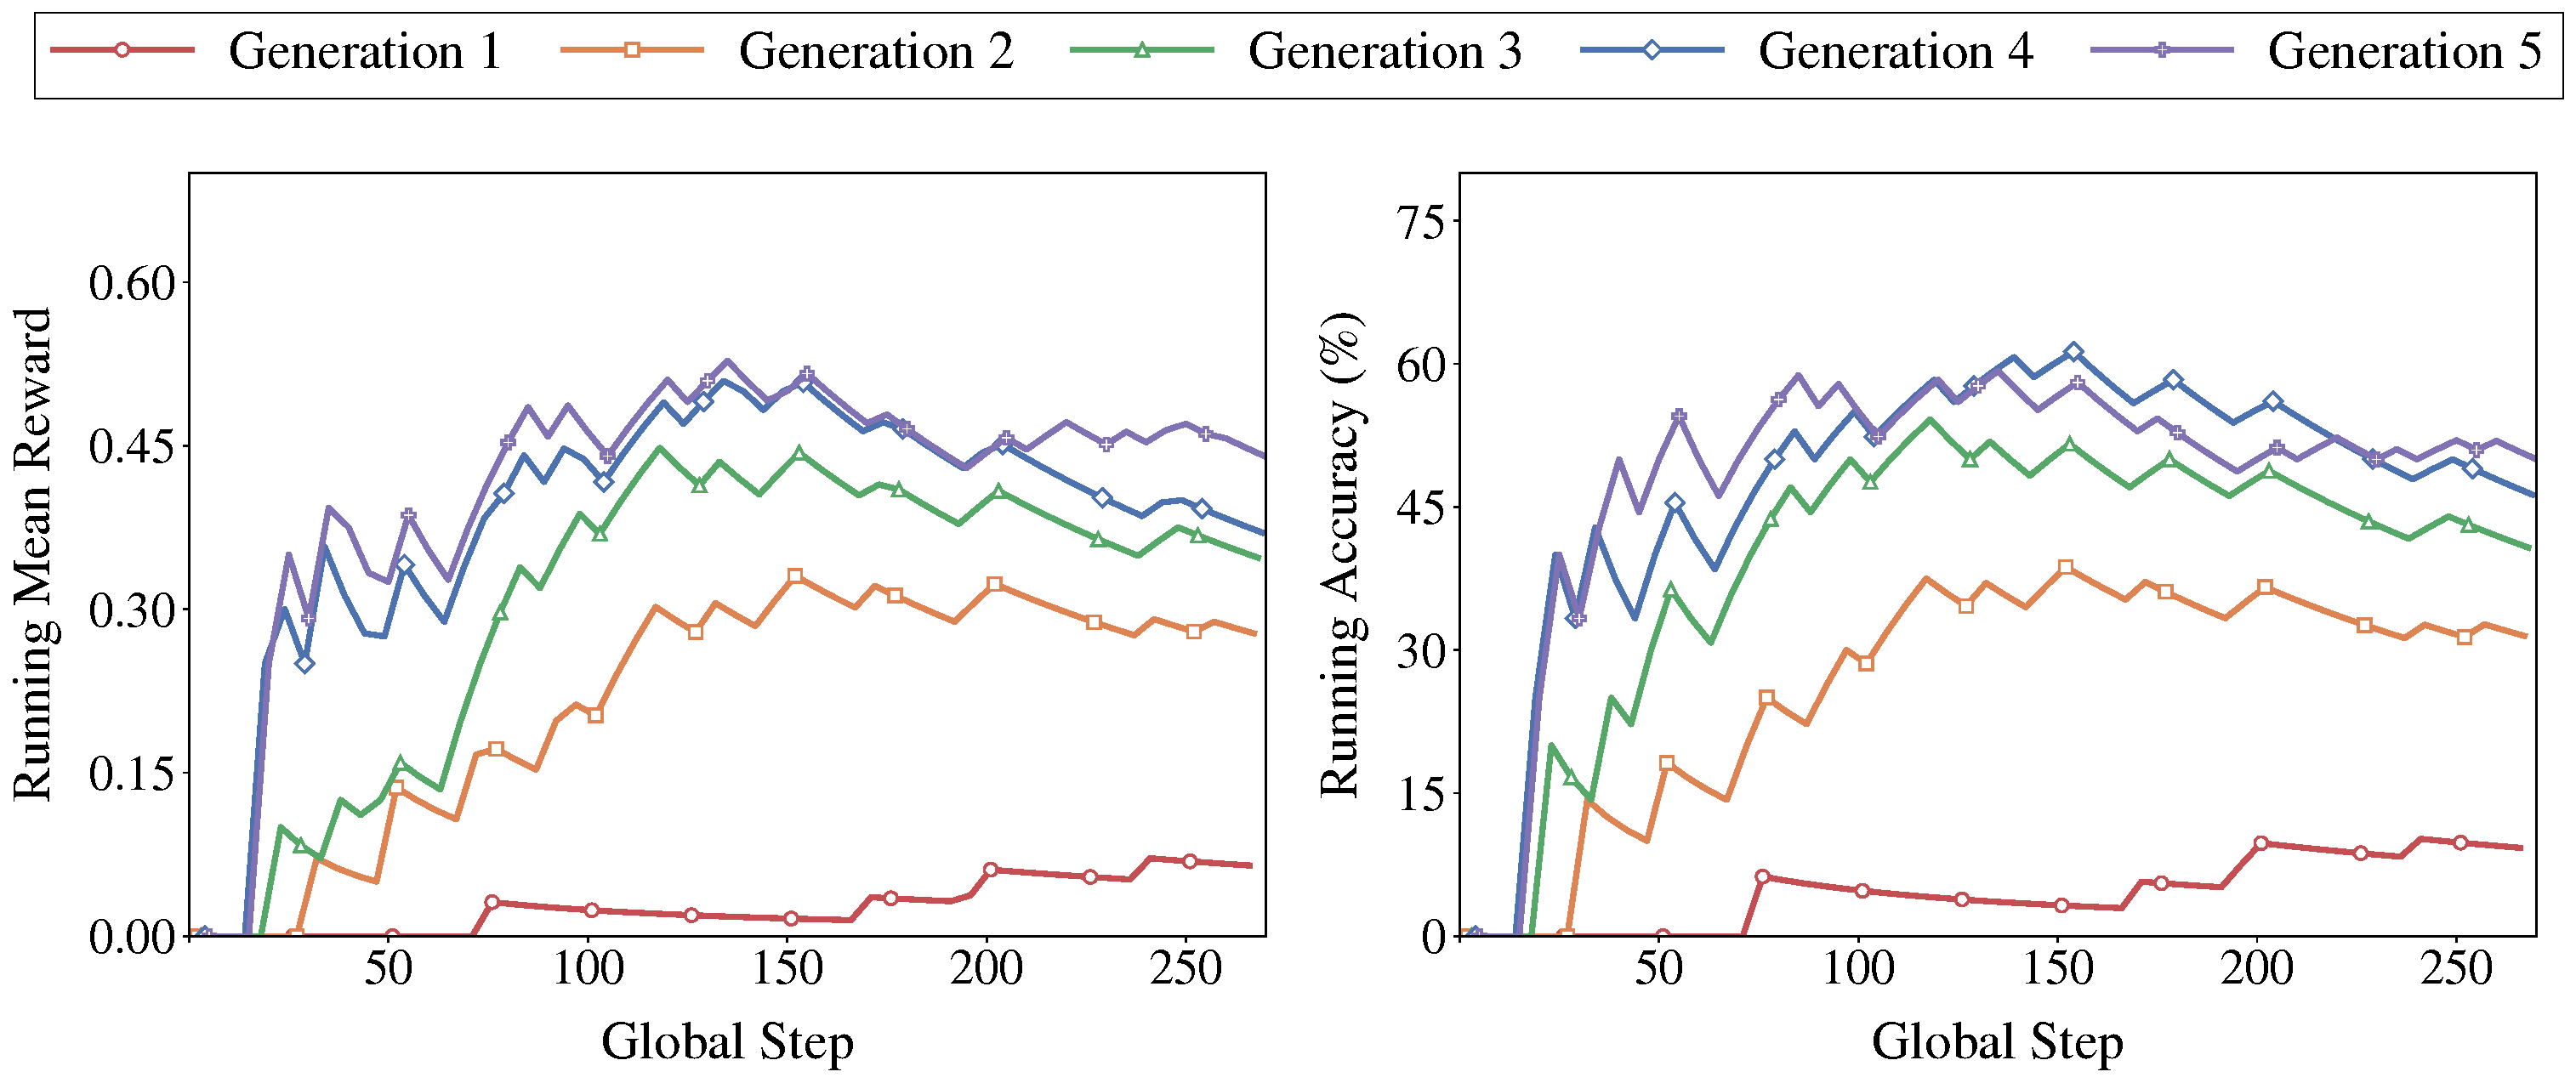
\includegraphics[width=\linewidth]{figures/combined_figure.pdf}
    % \caption{Accuracy across generations}
    % \label{fig:accuracy_per_gen}
    \caption{Accuracy and reward curves across 5 generations. }
    \label{fig:combined}
    \vspace{-1em}
\end{figure}

The two figures reveal a clear and largely monotonic ordering after the initial warm-up: Generation~5 outperforms Generation~4, which outperforms Generation~3, and so on, but the magnitude of improvement is not uniform across generations. The largest gains occur between Generations~1 and~3, where both reward and accuracy increase sharply as useful skills begin to transfer across tasks. By the end, Generation~5 reaches a running mean reward of $0.44$ and accuracy of $50.0\%$, compared to $0.06$ reward and $9.3\%$ accuracy for Generation~1, while Generation~4 achieves $0.37$ and $46.3\%$. This pattern suggests that most of the broad performance gains are realized by the first three generations, while Generations~4 and~5 increasingly plateau and primarily refine an already strong skill set rather than opening up a comparably new level of capability.

Comparing reward and accuracy further clarifies this behavior. The larger improvement in reward than accuracy from Generation~4 to~5 indicates that later generations improve consistency rather than merely solving additional tasks. Once a task becomes solvable, they increase the likelihood that sampled rollouts succeed, enhancing reliability within each task. The largest jump still occurs between the early generations, especially from Generation~1 to Generations~2 and~3, indicating that the highest-value skill repairs are discovered early. Later generations improve more modestly, but the accuracy panel shows that those improvements remain meaningful rather than cosmetic. This suggests that a small number of editing rounds captures the majority of improvements, with additional iterations yielding incremental but meaningful gains in robustness and coverage.

\subsection{Qualitative Analysis}
% \subsubsection{Trained v/s Inference Skill Editor}
% The performance gap between Skill-R1 (GRPO Editor) and Skill-R1 (Inference Editor) in \Cref{tab:main_results} reflects a deeper difference in what each editor learns to treat as signal. At a high level, the comparison is between two editing behaviors: one that treats rollout evidence as a cue for selective repair, and one that absorbs incidental context and drifts toward overfitting. The \texttt{pdb} skill is a useful lens on this distinction because it begins as a broad reference document, covering BioPython workflows, structure traversal, coordinate extraction, distance computation, ligand handling, and manual parsing. It is written as a general-purpose manual rather than a task-specific policy.

% When both editors are exposed to rollout evidence containing a genuine PDB failure together with unrelated nearby context, the trained editor responds conservatively. It preserves the basic structure of the skill, retains executable BioPython examples, and inserts targeted safeguards around actual failure points, such as missing dependencies, missing files, and empty models or chains. Even when the rollout contains evidence about misuse, that information remains peripheral. The resulting artifact is still recognizably a PDB skill: narrower and more robust than the original, but still broadly applicable to novel structure-analysis queries.

% The inference-only editor behaves very differently. Instead of repairing the skill while preserving its executable core, it rewrites the document around the incidental details of the sampled rollout. In the extreme case, it treats an internal benchmark identifier as though it were a malformed PDB accession and devotes substantial space to rejecting an unrelated audio query. The Quick Start and code examples disappear entirely, replaced by benchmark-shaped warnings and verbose instructions anchored to a small number of observed failures. The result is not a repaired skill but an overfit response policy whose content is dominated by accidental co-occurrence.

% This contrast clarifies why reward-trained editing outperforms inference-only editing. Without a cross-task reward signal, inference-time revision has no reliable mechanism for separating transferable structure from coincidental context. GRPO changes that inductive bias. Because the editor is optimized against bi-level advantages aggregated across rollouts, it is encouraged to preserve what continues to work across tasks and to modify only those parts of the skill that systematically limit reward. The learned behavior is therefore not simply ``more cautious'' editing; it is editing that is selective about what deserves to be remembered. Full skill listings for both the GRPO-edited and inference-edited \texttt{pdb} skill (alongside the original) are provided in \Cref{app:pdb_skill_comparison}.

% \subsubsection{Editing Trajectory Across Generations}
% Tracing the same skill across generations reveals a second qualitative pattern. Skill evolution is not a story of monotonic accumulation, where each round simply appends more advice to an already long document. Instead, the editor first compresses broad, tutorial-like skills into shorter executable routines, then sharpens them around recurrent failure modes, and finally stabilizes them with stronger task-boundary guardrails. The overall effect is a prune-then-specialize dynamic in which general reference material is gradually displaced by compact instructions that are easier to deploy under the distribution of tasks encountered during training.

% The \texttt{pdb} skill provides a concrete illustration of this progression. In its original form, the skill reads like a general-purpose reference manual, containing multiple BioPython workflows, file-format documentation, and manual parsing utilities. By the first generation, that broad reference has already been condensed into a single distance-computation workflow accompanied by a short list of concrete best practices. In the second generation, the skill narrows further: background exposition is stripped away, and the document is reorganized around local-file handling, explicit error checks, and tightly specified output behavior. By the third generation, the skill no longer resembles a general primer. It functions instead as a compact policy, retaining only a small executable core while adding stronger misuse guardrails, including an explicit rejection of an unrelated audio-file query. This complements the trained-vs.-inference comparison above. GRPO training curbs the most pathological forms of overfitting seen in inference-only editing, but it does not eliminate task conditioning altogether. Over longer horizons, the dominant trend is a shift away from general-purpose documentation and toward compact, deployment-oriented artifacts that increasingly reflect the recurrent structure of the training distribution. 

\subsubsection{Trained v/s Inference Skill Editor}

The performance gap between Skill-R1 (GRPO) and Skill-R1 (Inference) in \Cref{tab:main_results,tab:webwalker_results} reflects a fundamental difference in how each editor interprets rollout evidence. The trained editor treats rollouts as signals for targeted repair, while the inference-only editor tends to overfit to incidental context.

Using the \texttt{pdb} skill as a case study, the trained editor preserves the core executable structure and introduces focused safeguards around genuine failure modes (e.g., missing files or dependencies). In contrast, the inference-only editor rewrites the skill around spurious details from sampled rollouts, often discarding essential components such as executable code. This leads to brittle, task-specific artifacts that fail to generalize.

This qualitative difference is reflected in performance, while inference-only Skill-R1 provides modest gains over Vanilla GRPO on GAIA (30.9\% vs. 29.7\%), it underperforms on WebWalker (19.0\% vs. 22.0\%), the GRPO-trained editor consistently improves performance across benchmarks (41.8\% on GAIA and 26.0\% on WebWalker), demonstrating that reward driven editing better captures transferable structure.

Overall, training enables selective retention of useful behaviors while suppressing noise, leading to more robust and generalizable skill updates. Full skill listings for both the GRPO-edited and inference-edited \texttt{pdb} skill (alongside the original) are provided in \Cref{app:pdb_skill_comparison}.

\subsubsection{Editing Trajectory Across Generations}

Skill evolution follows a structured progression rather than simple accumulation. Early generations yield the largest gains by correcting high-impact errors, as also reflected in the sharp improvements from Generation 1 to 3 in \Cref{fig:combined}. Later generations provide smaller but consistent improvements by refining reliability and stabilizing behavior.

Qualitatively, this corresponds to a prune then specialize dynamic. Initial skills, which resemble broad reference documents, are quickly compressed into shorter executable routines. Subsequent generations focus on recurring failure modes and introduce tighter constraints and guardrails, resulting in compact, deployment oriented policies.

This pattern aligns with the quantitative trends: most performance gains are realized early, while later iterations primarily improve consistency rather than expanding capability. Together, these observations suggest that multi-generation evolution is effective not only for discovering better skills, but also for making them more reliable under repeated execution.
\section{Related Work}

\subsection{Agent Skill in Language Models}

% \begin{itemize}
%     \item \href{https://arxiv.org/pdf/2504.06821}{https://arxiv.org/pdf/2504.06821}
%     \item \href{https://arxiv.org/pdf/2602.02474}{https://arxiv.org/pdf/2602.02474}
%     \item \href{https://arxiv.org/pdf/2603.18743}{https://arxiv.org/pdf/2603.18743}
%     \item \href{https://www.arxiv.org/pdf/2602.08234}{https://www.arxiv.org/pdf/2602.08234}
%     \item \href{https://arxiv.org/pdf/2601.21557}{https://arxiv.org/pdf/2601.21557}
%     \item \href{https://arxiv.org/pdf/2308.00304}{https://arxiv.org/pdf/2308.00304}
%     \item \href{https://arxiv.org/pdf/2602.12430}{https://arxiv.org/pdf/2602.12430}
%     \item \href{https://arxiv.org/pdf/2504.06821}{https://arxiv.org/pdf/2504.06821}
%     \item \href{https://arxiv.org/pdf/2504.07079}{https://arxiv.org/pdf/2504.07079}
%     \item \href{https://arxiv.org/pdf/2601.21123}{https://arxiv.org/pdf/2601.21123}
%     \item \href{https://arxiv.org/pdf/2603.12056}{https://arxiv.org/pdf/2603.12056}
%     \item \href{https://arxiv.org/pdf/2602.02474}{https://arxiv.org/pdf/2602.02474}
%     \item \href{https://arxiv.org/pdf/2603.18743}{https://arxiv.org/pdf/2603.18743}
%     \item \href{https://arxiv.org/pdf/2603.25158}{https://arxiv.org/pdf/2603.25158}
%     \item \href{https://arxiv.org/pdf/2603.00718}{https://arxiv.org/pdf/2603.00718}
%     \item \href{https://arxiv.org/pdf/2512.17102}{https://arxiv.org/pdf/2512.17102}
% \end{itemize}

Recent work treats agent skills as reusable procedural abstractions that guide LLM behavior without modifying model parameters. Surveys (~\citep{xu2026agent},~\citep{jiang2026sok}) characterize skills as structured intermediates between tool usage and agent coordination. On the acquisition side, prior work has focused on constructing and organizing skill libraries~\citep{nguyen2025guisurvey, huang2025surveyfoundation}. SkillWeaver(~\citep{zheng2025skillweaver}) enables agents to autonomously discover and distill skills through web interaction, while ASI(~\citep{wang2025inducing}) shows that programmatic skill representations improve reliability via verifiability. Similarly, CUA-Skill~\citep{chen2026cua} introduces a repository of parameterized execution graphs for computer-use agents. Adjacent agentic-LLM work treats reusable procedures and contextual conditioning as central design tools for tool use, document reasoning, and multimodal interaction~\citep{xia2025sand, wu2025docreact,wu2025ctrls,wang2025dice,huang2025towardsagentic}. Other works study orchestration and system-level design ~\citep{li2026organizing}, which explores ecosystem-scale skill coordination. More recent efforts move beyond static skill banks toward skill evolution. MemSkill~\citep{zhang2026memskill} models memory operations as skills refined through iterative control loops, while Memento-Skills~\citep{zhou2025memento} enables continual skill improvement through reflective updates without modifying the base model. However, these approaches largely rely on heuristic refinement or implicit feedback signals.

\subsection{Reinforcement Learning for Language Models}

Reinforcement learning has become a central paradigm for aligning language models with task objectives and feedback signals. Methods such as PPO ~\citep{schulman2017proximal} and its variants optimize policies using scalar rewards, while more recent approaches like GRPO ~\citep{shao2024deepseekmath} introduce group-relative comparisons to stabilize training and improve sample efficiency. Recent variants further extend GRPO to weakly-supervised and reward-conditioned settings~\citep{mundada2026wsgrpo,zhong2026rc}. Several works extend RL to agent settings and skill learning. SkillRL~\citep{xia2026skillrl} jointly learns hierarchical skills and policies through recursive reinforcement learning, enabling agents to acquire reusable behaviors over time. Despite these advances, most existing methods focus on optimizing the task model itself or operate within a single-generation setting, limiting their ability to capture iterative improvement.


% Recent work treats skills as explicit, reusable procedural modules for LLM agents, rather than leaving all behavior implicit in model weights. This perspective appears in in-context skill elicitation for compositional reasoning~\citep{chen2024skills}, broader formulations of agent skills as a modular layer in LLM systems~\citep{xu2026agent}, and systems that acquire or organize skills as executable artifacts, such as programmatic skill induction, web-skill discovery, computer-use skill libraries, and skill-centric evaluation frameworks~\citep{wang2025programmaticskills,zheng2025skillweaver,chen2026cuaskill,chen2026skillcraft}.

% A second line of work studies how skills can be accumulated, distilled, and evolved over time, including memory skills, stateful skill memories, multimodal experience-and-skill learning, trajectory-to-skill distillation, and context-level skill evolution~\citep{zhang2026memskill,zhou2026mementoskills,jiang2026xskill,ni2026trace2skill,ye2026metacontext}. Some approaches further combine skill libraries with reinforcement learning for self-improvement~\citep{xia2026skillrl,wang2026selfimprovingagentskilllibrary}. In contrast, our work focuses on recurrent instance-level skill revision: we keep the task LLM frozen and optimize a separate skill generator to improve external skills across generations from verifier-scored rollouts.







% \note{Let's add related works here.}
% \href{https://arxiv.org/pdf/2504.06821}{Agent Skill Induction (ASI)} \textbf{COLM 2025}\\
% This paper introduces \textbf{Agent Skill Induction (ASI)}, a framework enabling
% web navigation agents to autonomously learn reusable skills represented as
% executable Python programs rather than free-form text. Given a natural language
% query $q$, the agent first generates an action trajectory
% $\tau = (s_0, a_0, s_1, a_1, \ldots, s_{H-1}, a_{H-1}, s_H)$ using primitive
% actions (e.g., \texttt{click}, \texttt{scroll}). ASI then abstracts recurring
% sub-sequences into higher-level programmatic skills (e.g.,
% \texttt{search\_product(name)}) and verifies them along three dimensions:
% (1)~\textit{Correctness}---whether executing the rewritten trajectory $\tau_f$
% solves the task as judged by an evaluator $V_L(e) \rightarrow \{0, 1\}$;
% (2)~\textit{Skill Usage}---whether $\tau_f$ contains at least one call to a
% newly induced skill $D$; and (3)~\textit{Skill Validity}---whether all
% skill-calling actions cause environment state changes. Only verified skills are
% added to the agent's action library $A_t \cup D_{\text{called}} \rightarrow
% A_{t+1}$. Unlike AWM, which augments agent memory via $M_t \cup \{d_t\}
% \rightarrow M_{t+1}$, ASI directly expands the action space. Evaluated on the
% \textbf{WebArena} benchmark, ASI outperforms the static baseline by
% $\mathbf{23.5\%}$ and the text-skill counterpart (AWM) by $\mathbf{11.3\%}$ in
% success rate, while reducing action steps by $10.7$--$15.3\%$ through
% composition of primitives into higher-level skills. The paper further
% demonstrates ASI's effectiveness in scaled-up browsing scenarios and
% cross-website skill transfer, where induced skills can be reused or updated to
% adapt to new website structures.

% \href{https://arxiv.org/pdf/2512.17102}{Reinforcement Learning for Self-Improving Agent with Skill Library} \textbf{AWS Agentic AI}\\
% This paper introduces \textbf{SAGE} (\textit{Skill Augmented GRPO for
% self-Evolution}), a reinforcement learning framework that enables LLM-based
% agents to continuously self-improve by learning, validating, and reusing
% executable programmatic skills stored in a skill library $\mathcal{M}$. Unlike
% prior skill library approaches that rely solely on LLM prompting, SAGE extends
% Group Relative Policy Optimization (GRPO) with two key components:
% (1)~\textit{Sequential Rollout}, which deploys agents across a chain of similar
% tasks $Q = \{q_1, q_2, \ldots, q_N\}$ within each rollout, allowing skills
% generated from earlier tasks to accumulate in $\mathcal{M}$ and become available
% for subsequent tasks; and (2)~\textit{Skill-integrated Reward}, which augments
% the standard outcome-based reward with an additional signal for high-quality
% skill generation and utilization. The agent follows a unified format (building on
% DynaSaur and CodeAct) where, during environment interaction, it generates
% reusable skill functions $\hat{a}$ composed of API calls, immediately executes
% them, and saves successful skills to the library via operations including
% \texttt{Skill Usage}, \texttt{Skill Generation}, \texttt{Skill Update}, and
% \texttt{Skill Save}. Skills are retrieved from $\mathcal{M}$ as a subset
% $[a_1, \ldots, a_k]$ and injected into context before each task. Evaluated on
% the \textbf{AppWorld} benchmark, SAGE applied to a supervised-finetuned
% Qwen2.5-32B-Instruct achieves $\mathbf{72.0\%}$ Task Goal Completion and
% $\mathbf{60.7\%}$ Scenario Goal Completion---an $8.9\%$ improvement in SGC over
% the baseline GRPO ($51.8\%$)---while requiring $26\%$ fewer interaction steps
% (12.1 vs.\ 16.4) and generating $59\%$ fewer tokens (1{,}475 vs.\ 3{,}613).
% Agents trained with SAGE also demonstrate more than $2\times$ success rate when
% utilizing learned skills compared to prompting-based approaches, confirming the
% effectiveness of RL-driven skill acquisition for continuous agent
% self-improvement.

% \href{https://arxiv.org/pdf/2602.02474}{MemSkill: Learning and Evolving Memory Skills for Self-Evolving Agents}\\
% This paper presents \textbf{MemSkill}, a framework that replaces the static,
% hand-designed memory operations in LLM agent systems with \textit{learnable and
% evolvable memory skills}---structured, reusable routines for extracting,
% consolidating, and pruning information from interaction traces. MemSkill
% comprises three core components: (1)~a \textit{controller} that learns to
% select a small subset of relevant skills from a shared skill bank given the
% current context; (2)~an LLM-based \textit{executor} that conditions on the
% selected skills to produce skill-guided memories in a single pass over each
% span of interaction history; and (3)~a \textit{designer} that periodically
% mines hard cases---instances where selected skills yield incorrect or
% incomplete memories---selects representative failures, and uses an LLM to
% refine existing skills and propose new ones. The system operates through a
% closed-loop optimization procedure that alternates between two phases:
% \textit{learning}, where the controller is trained via reinforcement learning
% with downstream task signals as reward feedback for skill selection, and
% \textit{evolution}, where the designer updates the skill bank based on
% accumulated difficult cases, with an optional rollback mechanism if updates
% cause regression. This skill-conditioned formulation is agnostic to a fixed
% extraction unit and generalizes across different span lengths when processing
% long interaction histories. MemSkill is evaluated on four benchmarks---LoCoMo,
% LongMemEval, HotpotQA, and ALFWorld---spanning conversational memory, long-term
% memory evaluation, multi-hop question answering, and embodied interactive
% decision-making. Results demonstrate that the learned and evolved skill bank
% enables more adaptive memory construction than static baselines, with the
% reusable skill bank additionally supporting transfer across datasets and base
% models.



% \subsection{Reinforcement Learning in Language Models}

% \begin{itemize}
% \item \href{https://arxiv.org/pdf/2203.02155}{https://arxiv.org/pdf/2203.02155}
% \item \href{https://arxiv.org/pdf/2402.03300}{https://arxiv.org/pdf/2402.03300}
% \item \href{https://arxiv.org/pdf/2501.12948}{https://arxiv.org/pdf/2501.12948}
% \item \href{https://arxiv.org/pdf/2503.23829}{https://arxiv.org/pdf/2503.23829}
% \item \href{https://arxiv.org/pdf/2506.14245}{https://arxiv.org/pdf/2506.14245}
% \item \href{https://arxiv.org/pdf/2509.16679}{https://arxiv.org/pdf/2509.16679}
% \item \href{https://arxiv.org/pdf/2507.04136}{https://arxiv.org/pdf/2507.04136}
% \item \href{https://arxiv.org/abs/2503.20783}{https://arxiv.org/abs/2503.20783}

% \end{itemize}
\section{Conclusion}
\label{sec:conclusion}
We presented Skill-R1, a framework for recurrent skill evolution that improves agent performance without modifying the underlying task model. By decoupling execution from skill refinement and introducing a bi-level optimization objective, Skill-R1 enables iterative, reward-driven improvement over multiple generations. Empirically, Skill-R1 consistently outperforms both no-skill baseline and standard GRPO across benchmarks, with the largest gains observed on complex, multi-step tasks. Analysis shows that early generations drive most capability improvements, while later iterations enhance reliability and consistency, highlighting the importance of both evolution and stabilization. Overall, our results suggest that skill evolution is a practical alternative to model-level adaptation, offering a lightweight yet effective mechanism for improving agent behavior in both open- and closed-source settings.
\textbf{LLM usage disclosure:} AI tools were used to assist creating illustrative figures. 
\footnote{Tong and Ryan contributed to the conceptual and methodological design and did not process, store, or direct the use of project models or data.}


\bibliography{colm2026_conference}
\bibliographystyle{colm2026_conference}

\appendix
% % =========================================================
% \section{MCMC View and Tracking Guarantees for Recurrent Skill Self-Sampling}
% \label{app:mcmc_view}

% This appendix provides formal statements supporting the MCMC interpretation in
% Section~\ref{sec:method-loop}. We emphasize that Skill-R1 does not enforce detailed balance, hence classical MCMC
% stationarity results do not directly apply. Instead, we provide (i) a stationary-limit corollary when parameters converge
% and (ii) a tracking bound that controls deviation from stationarity under bounded parameter drift.

% \subsection{Preliminaries and notation}
% Fix an instance $x$. Let $\mu_g$ denote the marginal distribution of the sampled skill $s_g$.
% We use $\|\cdot\|_{\mathrm{TV}}$ for total variation distance.
% When discussing a stationary distribution of a kernel, we use $\pi_\phi^\infty$ to denote any invariant distribution
% associated with a \emph{frozen} transition kernel parameterized by $\phi$.

% \subsection{Stationary-limit guarantee under parameter convergence}
% \label{app:stationary_limit}

% \begin{proposition}[Stationary-limit of skill sampling under parameter convergence]
% \label{prop:stationary_limit}
% Assume that for a fixed instance $x$, the skill generator parameters converge, i.e., $\phi_g \to \phi^\star$ as
% $g\to\infty$, and the mapping $\phi \mapsto \pi_\phi(\cdot \mid x,\mathcal{H})$ is continuous in total variation for any
% fixed $(x,\mathcal{H})$.
% Then the induced skill sampling distribution $\mu_g$ converges to a limiting distribution $\mu^\star$, and $\mu^\star$ is
% stationary with respect to the frozen proposal distribution $\pi_{\phi^\star}$ in the sense that repeated sampling from
% $\pi_{\phi^\star}(\cdot \mid x,\mathcal{H})$ yields the same marginal $\mu^\star$.
% \end{proposition}

% \begin{remark}
% Proposition~\ref{prop:stationary_limit} is a minimal but fully valid guarantee. It does not claim that the limit equals a
% Gibbs distribution of the form $\propto \exp(\beta J(s;x))$; it states that if learning stabilizes, the induced sampling
% stabilizes as well, which is the appropriate notion of stationarity for a learned proposal.
% \end{remark}

% \subsection{Tracking bound under bounded parameter drift}
% \label{app:tracking_bound}

% To connect with an MCMC-style notion of stationarity, consider a frozen generation-level transition kernel on skills
% $T_\phi$ (e.g., a one-step kernel that samples a skill according to the current proposal and returns it as the next state).
% Let $\pi_\phi^\infty$ denote an invariant distribution of $T_\phi$.

% \begin{assumption}[Uniform mixing of frozen kernels]
% \label{assump:mixing}
% For every $\phi$ in a neighborhood of the iterates, the frozen kernel $T_\phi$ is uniformly geometrically ergodic:
% there exist constants $C \ge 1$ and $\rho \in (0,1)$ such that for any initial distribution $\nu$,
% \begin{equation}
% \left\|\nu T_\phi^t - \pi_\phi^\infty \right\|_{\mathrm{TV}} \le C \rho^t \qquad \forall t \ge 0.
% \label{eq:geom_ergodic}
% \end{equation}
% \end{assumption}

% \begin{assumption}[Lipschitz dependence on parameters]
% \label{assump:lipschitz}
% There exists $L>0$ such that for all $\phi,\phi'$ in the same neighborhood,
% \begin{equation}
% \left\| \pi_\phi^\infty - \pi_{\phi'}^\infty \right\|_{\mathrm{TV}} \le L \|\phi-\phi'\|.
% \label{eq:lipschitz_inv}
% \end{equation}
% \end{assumption}

% \begin{theorem}[Stationary tracking under slow parameter drift]
% \label{thm:tracking}
% Assume Assumptions~\ref{assump:mixing}--\ref{assump:lipschitz}. Suppose the parameter updates satisfy a bounded drift
% condition $\|\phi_g - \phi_{g-1}\| \le \eta$ for all $g$.
% Then the deviation between the skill marginal $\mu_g$ and the invariant distribution of the frozen kernel satisfies
% \begin{equation}
% \left\|\mu_g - \pi_{\phi_g}^\infty \right\|_{\mathrm{TV}}
% \;\le\;
% C\rho \left\|\mu_{g-1} - \pi_{\phi_{g-1}}^\infty \right\|_{\mathrm{TV}}
% \;+\;
% L\eta.
% \label{eq:tracking_recursion}
% \end{equation}
% In particular, iterating \eqref{eq:tracking_recursion} yields the steady-state bound
% \begin{equation}
% \sup_g \left\|\mu_g - \pi_{\phi_g}^\infty \right\|_{\mathrm{TV}}
% \;\le\;
% \frac{L\eta}{1 - C\rho},
% \label{eq:tracking_bound}
% \end{equation}
% whenever $C\rho<1$.
% \end{theorem}

% \begin{remark}[Interpretation]
% Theorem~\ref{thm:tracking} provides a concrete and falsifiable statement: if the generator parameters change slowly
% (relative to mixing), then the actual skill sampling distribution tracks the stationary distribution of the corresponding
% frozen kernel, up to an error proportional to the per-generation drift $\eta$.
% This gives a formal sense in which a stationary distribution can be meaningfully discussed as an approximation, and it
% clarifies when an MCMC-inspired view is theoretically compatible with a learned, time-varying proposal.
% \end{remark}

% \paragraph{Proof sketch.}
% Let $\mu_g = \mu_{g-1} T_{\phi_g}$ denote one-step evolution under the current frozen kernel.
% Insert and subtract $\pi_{\phi_g}^\infty$ and use \eqref{eq:geom_ergodic} with $t=1$ to control contraction in total
% variation, yielding the first term in \eqref{eq:tracking_recursion}. The second term follows by adding and subtracting
% $\pi_{\phi_{g-1}}^\infty$ and applying \eqref{eq:lipschitz_inv} with $\|\phi_g-\phi_{g-1}\|\le \eta$.
% Iterating the recursion gives \eqref{eq:tracking_bound}.

% % =========================================================
% \section{Connections to GRPO Theory and Guarantees for Bi-Level Advantages}
% \label{app:grpo_bilevel_theory}

% This appendix formalizes how the proposed bi-level advantages relate to group-relative policy optimization (GRPO)
% and provides basic guarantees supporting their use under recurrent, non-stationary generations.
% GRPO replaces a learned critic with a prompt-group baseline to reduce variance while preserving a valid policy-gradient
% update \cite{Shao2024DeepSeekMath}. Our intra-generation advantage follows this principle.
% Our inter-generation advantage addresses distribution drift induced by recurrent self-sampling across generations, a regime
% where baseline estimation is known to become unstable \cite{Wang2025KRPO}.

% \subsection{Setup}
% Fix an instance $x$ and generation $g$ with skill $s_g \sim \pi_\phi(\cdot\mid x,\mathcal H_{g-1})$ and rollouts
% $y^{(g,i)} \sim \pi_{\mathrm{task}}(\cdot\mid x,s_g)$ for $i=1,\dots,K$.
% Let $r^{(g,i)} := r(y^{(g,i)})$ and $\bar r_g := \frac{1}{K}\sum_{i=1}^K r^{(g,i)}$.

% We write the skill-conditioned expected reward as
% \begin{equation}
% J(s;x) := \mathbb{E}_{y \sim \pi_{\mathrm{task}}(\cdot\mid x,s)}[r(y)].
% \end{equation}
% We also define the induced objective of the skill generator under history $\mathcal H_{g-1}$:
% \begin{equation}
% \mathcal{J}_g(\phi;x) := \mathbb{E}_{s \sim \pi_\phi(\cdot\mid x,\mathcal H_{g-1})}[J(s;x)].
% \end{equation}

% \subsection{Intra-generation advantage as a control variate}
% Define the intra-generation advantage
% \begin{equation}
% A_{\mathrm{intra}}(y^{(g,i)}) := r^{(g,i)} - \bar r_g.
% \end{equation}
% By construction, it is centered within the generation:
% \begin{equation}
% \sum_{i=1}^K A_{\mathrm{intra}}(y^{(g,i)}) = 0.
% \label{eq:zero_sum_intra}
% \end{equation}

% \begin{proposition}[Centered group baselines preserve the policy gradient]
% \label{prop:control_variate}
% Assume $\pi_{\mathrm{task}}$ and $r$ do not depend on $\phi$. Then for any measurable baseline $b_g$ that is a function of
% $\{r^{(g,i)}\}_{i=1}^K$ but is independent of the sampled skill $s_g$ given $(x,\mathcal H_{g-1})$, the estimator
% \[
% \widehat{\nabla}_\phi \mathcal{J}_g(\phi;x)
% =
% \left(\frac{1}{K}\sum_{i=1}^K (r^{(g,i)} - b_g)\right)\nabla_\phi \log \pi_\phi(s_g\mid x,\mathcal H_{g-1})
% \]
% is an unbiased estimator of $\nabla_\phi \mathcal{J}_g(\phi;x)$.
% In particular, choosing $b_g=\bar r_g$ yields an unbiased gradient estimator with reduced variance compared to $b_g=0$.
% \end{proposition}

% \paragraph{Proof sketch.}
% Condition on $(x,\mathcal H_{g-1})$. Since $r^{(g,i)}$ depends on $\phi$ only through $s_g$, REINFORCE gives
% $\nabla_\phi \mathcal{J}_g(\phi;x) = \mathbb{E}[\bar r_g \nabla_\phi \log \pi_\phi(s_g\mid x,\mathcal H_{g-1})]$.
% Subtracting any baseline independent of $s_g$ leaves the expectation unchanged.

% \subsection{Inter-generation progress as a drift-sensitive statistic}
% Define the inter-generation advantage
% \begin{equation}
% A_{\mathrm{inter}}(g) := \bar r_g - \bar r_{g-1}.
% \end{equation}
% This quantity estimates the progress in the induced rollout population quality between successive generations.

% \begin{assumption}[Bounded rewards]
% \label{assump:bounded_rewards}
% $r(y)\in[0,R_{\max}]$ for all $y$.
% \end{assumption}

% \begin{assumption}[Controlled per-generation drift in skill quality]
% \label{assump:drift}
% There exists $\Delta \ge 0$ such that for all generations,
% \[
% \left|J(s_g;x) - J(s_{g-1};x)\right| \le \Delta
% \quad \text{almost surely.}
% \]
% \end{assumption}

% \begin{lemma}[Concentration of inter-generation progress]
% \label{lem:inter_concentration}
% Under Assumption~\ref{assump:bounded_rewards}, for any fixed $g$ and $\delta\in(0,1)$,
% \[
% \left|A_{\mathrm{inter}}(g) - \left(J(s_g;x)-J(s_{g-1};x)\right)\right|
% \le
% 2R_{\max}\sqrt{\frac{\log(2/\delta)}{2K}}
% \]
% with probability at least $1-\delta$ (over sampling of rollout populations in generations $g$ and $g-1$).
% \end{lemma}

% \paragraph{Proof sketch.}
% Apply Hoeffding's inequality to $\bar r_g$ and $\bar r_{g-1}$ separately and union bound.

% \begin{remark}[Why this is relevant to GRPO-style instability]
% Baseline mis-estimation becomes more severe when reward statistics drift rapidly across iterations, motivating dynamic
% baseline tracking mechanisms \cite{Wang2025KRPO}. Lemma~\ref{lem:inter_concentration} shows that $A_{\mathrm{inter}}(g)$
% is a statistically well-behaved progress estimator whose noise decays as $O(K^{-1/2})$ even under non-stationarity.
% \end{remark}

% \subsection{A theory-friendly bi-level objective}
% A key structural property used by group-relative objectives is that weights are centered within each prompt-group, which
% yields stable updates and (in some frameworks) cancels terms tied to normalization constants \cite{Zhang2025GVPO}.
% To preserve this property, we recommend using a decomposed bi-level objective:
% \begin{equation}
% \mathcal{L}_{\mathrm{bi}}(\phi)
% =
% \mathbb{E}_{x\sim\mathcal D}
% \left[
% \sum_{g=1}^G
% \Big(
% \underbrace{\sum_{i=1}^K A_{\mathrm{intra}}(y^{(g,i)})}_{\text{centered within generation}}
% \;+\;
% \lambda \underbrace{A_{\mathrm{inter}}(g)}_{\text{progress}}
% \Big)
% \log \pi_\phi(s_g\mid x,\mathcal H_{g-1})
% \right].
% \label{eq:bilevel_loss_skill_level}
% \end{equation}
% This form treats both signals as skill-level weights, consistent with the fact that only the skill generator is trained.
% Moreover, centering within generation remains explicit via \eqref{eq:zero_sum_intra}.

% \begin{proposition}[Bi-level update as an ascent direction with bounded perturbation]
% \label{prop:bilevel_ascent}
% Assume $\pi_{\mathrm{task}}$ and $r$ do not depend on $\phi$, and Assumption~\ref{assump:bounded_rewards} holds.
% Then the stochastic gradient of \eqref{eq:bilevel_loss_skill_level} is an ascent direction for the per-generation objective
% $\mathcal{J}_g(\phi;x)$ up to an additive perturbation term of magnitude $O(\lambda K^{-1/2})$ due to estimation noise in
% $A_{\mathrm{inter}}(g)$, controlled by Lemma~\ref{lem:inter_concentration}.
% \end{proposition}

% \paragraph{Proof sketch.}
% The intra term yields an unbiased REINFORCE estimator (Proposition~\ref{prop:control_variate}).
% The inter term depends only on generation-level sample means and thus contributes a bounded extra weight on
% $\nabla_\phi\log\pi_\phi(s_g\mid\cdot)$. Apply Lemma~\ref{lem:inter_concentration} to bound its deviation from the
% population progress $J(s_g;x)-J(s_{g-1};x)$.

% \subsection{Relation to recent GRPO extensions}
% Recent GRPO extensions add additional structure to recover learning signals in challenging regimes and provide theoretical
% analyses in stylized settings \cite{Chen2025SGPO}, or provide robustness/generalization guarantees when intermediate
% supervision is unavailable \cite{Mundada2025WSGRPO}. Our bi-level construction is complementary: it keeps the GRPO
% intra-group centering but adds an explicit progress statistic to stabilize recurrent, generation-indexed self-sampling.

% =========================================================

\section{Appendix}

\subsection{PDB Skill}
\label{app:pdb_skill_comparison}

This appendix provides the complete content of the \texttt{pdb} skill at three points in time, as referenced in \Cref{sec:analysis}: (1) the original skill from the shared skill library, (2) the version produced by the GRPO-trained Qwen3-4B editor after three generations of evolution (run \texttt{20260320\_131744\_0.25}), and (3) the version produced by the untrained base Qwen3-4B model operating in inference mode (run \texttt{20260321\_185812}).

% -----------------------------------------------------------
\subsubsection{Original \texttt{pdb} Skill}

The original skill is a general-purpose reference covering BioPython's full API. We reproduce the header description and the Quick Start section to illustrate the skill's initial breadth; the remainder of the document (Dependencies, PDB File Format Basics, Python Libraries, Manual Parsing, Common Tasks, Quick Reference table) is analogous in scope.

\begin{small}
\begin{verbatim}
name: pdb
description: Use this skill whenever the user wants to read, parse, analyze,
  or manipulate PDB (Protein Data Bank) files. This includes extracting atomic
  coordinates, analyzing protein structures, identifying residues, chains,
  ligands, computing distances between atoms, visualizing molecular structures,
  and converting between molecular file formats. If the user mentions a .pdb
  file or asks about protein/molecular structure data, use this skill.

# PDB (Protein Data Bank) File Processing Guide

## Quick Start

```python
from Bio.PDB import PDBParser

parser = PDBParser(QUIET=True)
structure = parser.get_structure("protein", "structure.pdb")

# Iterate through the hierarchy: Structure -> Model -> Chain -> Residue -> Atom
for model in structure:
    for chain in model:
        print(f"Chain {chain.id}: {len(list(chain.get_residues()))} residues")
```

## PDB File Format Basics

PDB files are fixed-width text files. Key record types:
| ATOM   | Standard residue atom coordinates  |
| HETATM | Non-standard residue (ligands, water) |
| SEQRES | Full sequence of residues          |
| REMARK | Comments and metadata              |

[... BioPython parsing examples, distance computation, ligand extraction,
     sequence extraction, manual ATOM-record parsing, and quick-reference
     table omitted for brevity -- all preserved in the original file ...]
\end{verbatim}
\end{small}

% -----------------------------------------------------------
\subsubsection{GRPO-Trained Editor: Edited \texttt{pdb} Skill}

\begin{small}
\begin{verbatim}
name: pdb
description: [unchanged from original]

# PDB (Protein Data Bank) File Processing Guide

## Quick Start

```python
from Bio.PDB import PDBParser
import numpy as np

# Parse a local PDB file path -- ensure the file exists at the specified path
parser = PDBParser(QUIET=True)

try:
    structure = parser.get_structure("structure", "5wb7.pdb")
except FileNotFoundError:
    print("Error: The PDB file was not found. Please verify the file name.")
    raise
except ImportError:
    print("Error: BioPython is not installed. pip install biopython")
    raise

# Access the first model and chain
models = list(structure)
if not models:
    raise ValueError("No models found in the PDB structure.")
model = models[0]

chains = list(model.get_chains())
if not chains:
    raise ValueError("No chains found in the model.")
chain = chains[0]

residues = list(chain.get_residues())
if not residues:
    raise ValueError("No residues found in the chain.")
```

## Common Misuse and Error Prevention

Note: This skill is for PDB files only. If the user provides an audio
recording (e.g., .mp3), it cannot be processed here.
\end{verbatim}
\end{small}

% -----------------------------------------------------------
\subsubsection{Base Inference Editor: Edited \texttt{pdb} Skill}

The untrained base Qwen3-4B model replaces the entire skill with the following. No executable code remains. The ``Key Requirements'' section mistakenly names the GAIA task UUID \texttt{7dd30055-0198-452e-8c25-f73dbe27dcb8} as an invalid PDB identifier, and the ``Common Misuse'' section is wholly devoted to handling a calculus homework audio recording (\texttt{Homework.mp3}) that is unrelated to PDB processing.

\begin{small}
\begin{verbatim}
name: pdb
description: [unchanged from original]

# PDB (Protein Data Bank) File Processing Guide

## Key Requirements and Best Practices

- Always ensure the PDB ID is valid and accessible via the RCSB PDB database.
- Use the correct PDB ID (e.g., "5wb7", not
  "7dd30055-0198-452e-8c25-f73dbe27dcb8") -- the latter is a UUID or
  invalid identifier.
- This skill does NOT handle audio files. If a user provides an audio file
  (e.g., Homework.mp3) and asks for page numbers, this skill is NOT applicable.

## Common Misuse and Clarifications

- Do not use this skill to extract page numbers from audio recordings.
- Do not attempt to parse audio files as if they were PDB files.
- If a user asks about study materials from a lecture, state that the skill
  cannot process audio content.
- Always verify the nature of the input: if it is .mp3 or .wav, respond with:
  "I cannot extract page numbers from audio files."

## Example of Incorrect Use

User: "I have a file called Homework.mp3 with my professor reading the
       recommended pages. Can you tell me the page numbers?"
Correct response: "I cannot extract page numbers from audio files. This skill
  is designed for processing PDB files, not audio recordings."

[--- No code examples remain in the edited skill ---]
\end{verbatim}
\end{small}

The contrast is stark. The GRPO-trained editor adds \emph{code} that handles real failure modes---a missing file, a missing library---while preserving the entire original reference. The base inference editor removes all code and fills the skill with content copied from two specific benchmark questions, leaving it useless for any unseen PDB task.

\end{document}
